\section{Kworkflow}

\texttt{Kworkflow}~\cite{kworkflow} (kw) is a \textit{Developer Automation
Workflow System} (DAWS) that targets Linux kernel developers. kw is a FLOSS
project licensed under the \textit{GNU General Public License version 2}
(GPLv2).

Generally, any developer who needs to work with the Linux source code can
benefit from using kw. For instance, in the GNU/Linux distribution (also called
\textit{distro}) layer, distro developers feed off the official releases (the
\textit{upstream} git repository) and maintain their own kernel tree (a
\textit{downstream} git repository) where they add their specific modifications
to the source code, occasionally returning contributions to the upstream. No
matter if they engage or not in the Linux project development, these developers
must also configure, build, deploy, and the like, making kw an interesting
choice.

kw aims to streamline and automate kernel workflows by offering a diverse set of
commands in a unified CLI that helps users to manage \texttt{.config} files,
build and deploy kernels, manage virtual and network-accessible machines,
seamlessly send patches in compliance with Linux guidelines, and more. Through
Bash script, kw leverages the \textit{GNU coreutils} and other CLI tools to
create solutions with sane basic configurations that offer a
\textit{plug-n-play} experience without limiting customization.

\subsection{Installation}

Currently, the best way to install kw is by cloning the project locally with
\texttt{git} and running the \texttt{setup.sh} script~\cite{kworkflow-setup}
with the \texttt{--install} option. After running the script, the user will be
prompted for superuser credentials to install the necessary dependencies using
the appropriate package manager (\texttt{apt}, \texttt{pacman}, \texttt{dnf},
etc.), then the script installs kw files in the user's system. \textbf{Listing
\ref{lst:kw-setup}} illustrates the mentioned steps.

\begin{lstlisting}[caption={Installing kw via the \texttt{setup.sh} script.}, label={lst:kw-setup}]
$ git clone https://github.com/kworkflow/kworkflow
$ cd kworkflow
$ ./setup.sh --install
\end{lstlisting}

\subsection{Features}

Once installed, kw offers a significant number of commands (features) that can
be invoked as described in \textbf{Listing \ref{lst:kw-commands}}. Features of
kw can be categorized depending on their purpose, and \textbf{Table
\ref{tab:kw-commands}} lists all features with their categories and
descriptions.

\begin{lstlisting}[caption={kw commands invocation.}, label={lst:kw-commands}]
$ kw <command> <options/arguments>
\end{lstlisting}

\begin{table}[ht]
    \caption{kw commands}
    \label{tab:kw-commands}
    \begin{center}
    \begin{tabular}{|p{0.2\columnwidth}|p{0.30\columnwidth}|p{0.40\columnwidth}|}
        \hline
        \rowcolor{gray!20}
        \textbf{Command} & \textbf{Category} & \textbf{Description} \\\hline
        \texttt{build}    & kernel build/deploy    & Build kernel and modules \\\hline
        \texttt{deploy}    & kernel build/deploy    & Deploy kernel and modules \\\hline
        \texttt{kernel\-config\-manager}    & kernel build/deploy    & Manage \texttt{.config} files \\\hline
        \texttt{env}    & kernel build/deploy    & Manage different environments for same kernel tree \\\hline
        \texttt{bd}    & kernel build/deploy    & Build and Deploy kernel and modules \\\hline
        \texttt{send-patch}    & patch submission    & Send patches via email \\\hline
        \texttt{maintainers}    & patch submission    & \texttt{get\_maintai\-ners.pl} wrapper \\\hline
        \texttt{codestyle}    & patch submission    & \texttt{checkpatch.pl} wrapper \\\hline
        \texttt{remote}    & target machine    & Manage machines in the network \\\hline
        \texttt{vm}    & target machine    & QEMU wrapper \\\hline
        \texttt{ssh}    & target machine    & \texttt{ssh} wrapper \\\hline
        \texttt{device}    & target machine    & Show hardware information \\\hline
        \texttt{debug}    & code inspection    & Linux debug utilities \\\hline
        \texttt{explore}    & code inspection    & Explore string patterns \\\hline
        \texttt{diff}    & code inspection    & Diff files \\\hline
        \texttt{init}    & kw management    & Initialize kw kernel tree \\\hline
        \texttt{config}    & kw management    & Set kw configs \\\hline
        \texttt{self-update}    & kw management    & Self-update mechanism \\\hline
        \texttt{backup}    & kw management    & Save and restore kw data \\\hline
        \texttt{clear-cache}    & kw management    & Clear kw cache \\\hline
        \texttt{patch-hub}    & misc    & TUI for patches from lore.kernel.org \\\hline
        \texttt{drm}    & misc    & DRM specific utilities \\\hline
        \texttt{pomodoro}    & misc    & Pomodoro technique \\\hline
        \texttt{report}    & misc    & Show usage statistics \\\hline
    \end{tabular}
    \end{center}
\end{table}

In the remainder of this section, we will deep dive into some of the kw
features, their use cases and highlight interesting aspects of each.
Nevertheless, \textbf{keep in mind} that kw does a lot more than what is
showcased next.

\subsubsection{kw build}

The \texttt{build} command, along with \texttt{deploy}, are the flagship
features of kw and probably the most elaborate ones. As mentioned in
\textbf{Section~\ref{sec:background:linux-tasks}}, building a kernel is not an
easy task, even when you have a \texttt{.config} ready. \textit{GNU make} (the
\texttt{make} utility) immensely helps in this task; nevertheless, one would
still have to keep in mind the target architecture, cross-compilation (if
needed), the number of CPU cores allocated, which \texttt{KCFLAGS} (short for
\textit{kernel compiler flags}) to use, and so on.

\begin{lstlisting}[caption={Example of kernel build \texttt{make} command.}, label={lst:classic-build-example}]
$ make ARCH=arm64 CROSS_COMPILE=aarch64-linux-gnu- -j8 'KCFLAGS=-DNICE_MACRO'
\end{lstlisting}

For instance, say the user wishes to build a kernel from an x86\_64 host to an
ARM64 target machine using all his CPU cores (eight cores available) while
defining a macro called \texttt{NICE\_MACRO}. Assuming that the necessary
\texttt{.config} is in place, \textbf{Listing~\ref{lst:classic-build-example}}
shows a \texttt{make} command for this scenario. 


In comparison, after a one-time simple setting of the aforementioned information
using the kw command \texttt{config} (as it will be described), the user only
needs to issue the command in \textbf{Listing~\ref{lst:kw-build-example}}.

\begin{lstlisting}[caption={\texttt{kw build} use case.}, label={lst:kw-build-example}]
$ kw build
\end{lstlisting}

The \texttt{build} command offers many options that go beyond simply automating
the equivalent \texttt{make} commands, namely: \texttt{--info} that displays
information about the current compilation with kernel name and number of modules
to be compiled; \texttt{--llvm} that enables use of the LLVM toolchain; and
\texttt{--from-sha} that builds every commit version of the kernel from a
\texttt{git} reference passed as an argument.

\subsubsection{kw deploy}

Although much less demanding regarding resources than building, deploying a
kernel can be more complicated and detail-filled than compiling. Simply put, the
task involves copying the necessary compiled artifacts to the correct place with
the correct name in the target machine's filesystem, defining a temporary
filesystem needed for the kernel to boot the system, and updating the
bootloader. Apart from these being non-trivial steps, these steps can also
mutate quite a lot depending on the target machine CPU architecture, Linux
distro, and many other factors.

The \texttt{deploy} command absorbs most of these complexities in its code, so
users do not need to configure most of the steps, with the feature detecting
information about the target machine and resolving the details. Unlike the pair
of \textbf{Listing~\ref{lst:classic-build-example}} and
\textbf{Listing~\ref{lst:kw-build-example}}, an equivalent series of commands
that would represent a single \texttt{kw deploy} call would involve many
commands (in the range of dozens) that are extensive, so presenting a comparison
here would only produce visual pollution. This speaks in favor of how well
\texttt{deploy} not only automates but streamlines the task of installing
kernels.\looseness=-1

Like with \texttt{build}, \texttt{deploy} has options that offer other
enhancements, like: \texttt{--list} to list installed kernels in a target
machine; \texttt{--uninstall} to uninstall kernels and related artifacts; and
\texttt{--create\-package} and \texttt{--from-package} to generate a compressed
file that can be transported offline (in a USB device, for instance) and be used
to deploy the kernel on another machine, which only has to have kw installed.\looseness=-1

\subsubsection{bd}

Because deploying a kernel often comes right after building it, kw offers the
\texttt{bd} command (from \textit{build and deploy}) to chain the two previously
mentioned features, optimizing even more the task of booting a kernel built from
the source code.

\subsubsection{kernel-config-manager}

Automating and streamlining the automation of a \texttt{.config} file that is
the perfect fit for a developer use case is an open problem, with some attempts
to solve this in the context of Linux CI~\cite{yildiran2024maximizing}. As such,
kw still does not cover the generation part, but offers a very comprehensive
feature, \texttt{kernel\-config-manager}, for users to easily keep records of a
great variety of \texttt{.config} files. The feature works differently depending
on the subcommand used: \texttt{--save} saves the current \texttt{.config} with
a name and an optional description; \texttt{--get} restores a saved
\texttt{.config} of the name passed as argument; and \texttt{--remove} removes
the entry related to the name passed as argument.

\begin{lstlisting}[caption={\texttt{kw kernel-config-manager} use case.}, label={lst:kw-k-example}]
$ kw k --save foo --description 'bar'
$ kw k --get foo
$ kw k --remove foo
\end{lstlisting}

\textbf{Listing~\ref{lst:kw-k-example}} exemplifies these three subcommands
usage (note that we use the short name \texttt{k} of the feature for
readability). \textbf{Figure 5} is a screen capture that showcases another
subcommand, \texttt{--list}, that lists all \texttt{.config} files managed by
the feature.

\begin{figure}[htbp]
    \centering
    \fbox{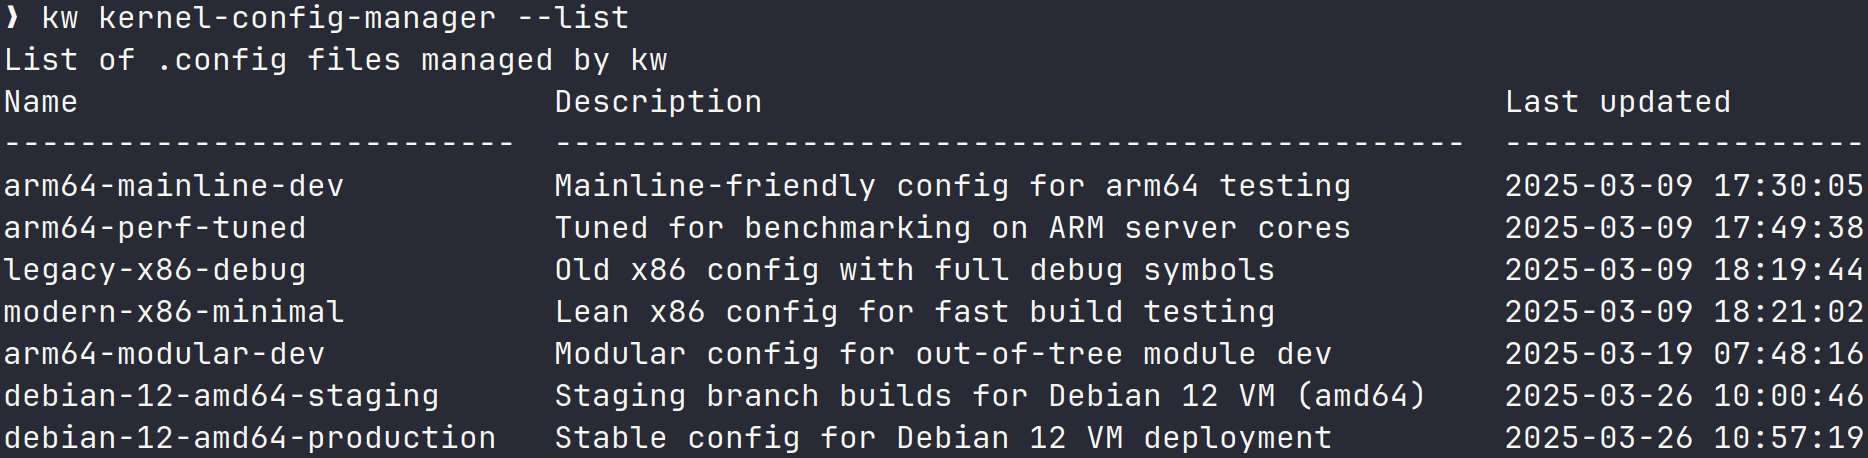
\includegraphics[width=1\linewidth, 
    clip=true, trim= 0px 0px 0px 0px]
    {figs/kw_k_list_example}}
    \caption{\texttt{kw kernel-config-manager --list} example.}
    \label{fig:patchset-dev-workflow}
\end{figure}

\subsubsection{env}

The result of building the kernel, i.e., the object files and related artifacts,
by default, resides in the same kernel tree used for the source code of the
compilation. However, some developers need to build kernels for different
targets from the same kernel tree, which becomes unmanageable as the number of
targets rises, due to the need for multiple \texttt{.config} files, build
configurations, and more.\looseness=-1

\begin{lstlisting}[caption={\texttt{kw env} use case.}, label={lst:kw-env-example}]
$ kw env --create FOO
$ kw env --use FOO
$ kw env --destroy FOO
\end{lstlisting}

To solve this problem, the \texttt{env} command allows users to create different
environments that isolate development contexts using a single kernel tree. The
corresponding files are stored inside a cache directory that is managed by kw.
With the use of the subcommands \texttt{--create}, \texttt{--use}, and
\texttt{--destroy}, users can manage their environments
(\textbf{Listing~\ref{lst:kw-env-example}}), and with \texttt{--list} consult
their environments (\textbf{Figure 6}).

\begin{figure}[htbp]
    \centering
    \fbox{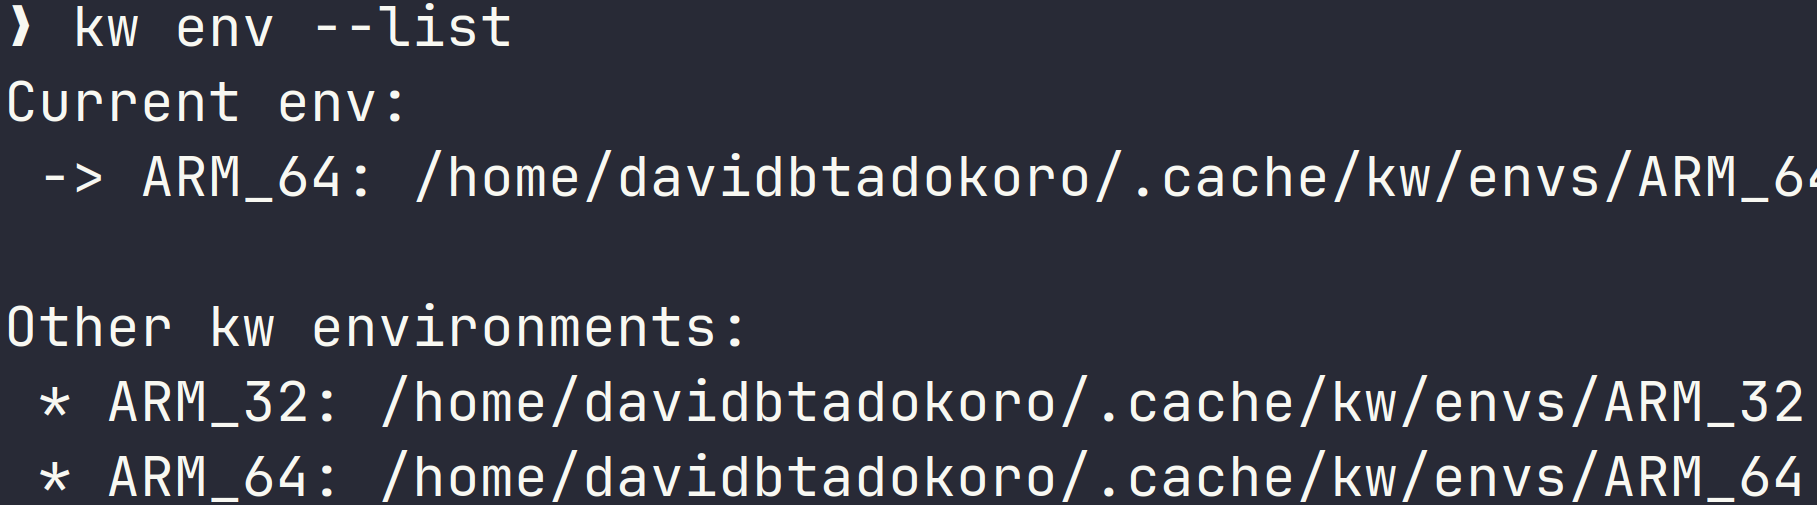
\includegraphics[width=0.8\linewidth, 
    clip=true, trim= 0px 0px 0px 0px]
    {figs/kw_env_list_example}}
    \caption{\texttt{kw env --list} example.}
    \label{fig:patchset-dev-workflow}
\end{figure}

\subsubsection{send-patch}

The act of converting a commit or set of commits into patches and sending them
through email is vastly covered by the \texttt{git-send-email} tool. However, it
can be considered raw from the point of needing a lot of configuration, verbose
commands, and, mainly, a lack of integration with the
\texttt{get\_maintainers.pl} tool. This last problem forces users to manually
resolve and add the correct recipients. The \texttt{send-patch} command solves
all three by providing default base configurations, shorter commands, and
automatically resolving recipients.
\textbf{Listings~\ref{lst:git-send-email-example}} and
\textbf{\ref{lst:kw-send-patch-example}} show, respectively, a
\texttt{git-send-email} command to send the current commit explicitly stating
the recipients with additional options and the respective \texttt{send-patch}
command.

\begin{lstlisting}[caption={Example of \texttt{git-send-email} command.}, label={lst:git-send-email-example}]
$ git send-email -1 --annotate --to=foo@bar.com --cc=bar@foo.com
\end{lstlisting}

\begin{lstlisting}[caption={\texttt{kw send-patch} use case.}, label={lst:kw-send-patch-example}]
$ kw send-patch --send
\end{lstlisting} 

\subsubsection{config}

Having a plethora of features, kw has its own system to manage the
configurations of each and a dedicated feature for users to interface with. The
syntax of the \texttt{config} feature is composed of the pair
\texttt{feature.configuration} followed by the value wished to be bound to the
configuration. For example, \textbf{Listing~\ref{lst:kw-config-example}}
illustrates a case of configuring the target architecture of the \texttt{build}
command to be x86\_64.

\begin{lstlisting}[caption={\texttt{kw config} use case.}, label={lst:kw-config-example}]
$ kw config build.arch 'x86_64'
\end{lstlisting}

\subsubsection{patch-hub}

A singular feature of kw is \texttt{patch-hub} as it is a sub-project with a
dedicated git repository, is written in Rust, and is a \textit{Terminal User
Interface} (TUI), a text-based equivalent of a \textit{Graphical User Interface}
(GUI) which significantly diverges from the fully CLI approach of the rest of
kw. Nonetheless, it still provides interesting services to kernel developers,
specifically the maintainers, as the feature is a TUI that allows users to
consult the flow of patches in lore.kernel.org, apply actions on them using
other kw features, and more. The feature aims to cover the patchset reviewing
workflow described in \textbf{Figure 2}. \texttt{patch-hub} has a lot more
capabilities and is a work-in-progress, but \textbf{Figure 5} gives an overview
of the potential of the feature.

\begin{figure}[htbp]
    \centering
    \fbox{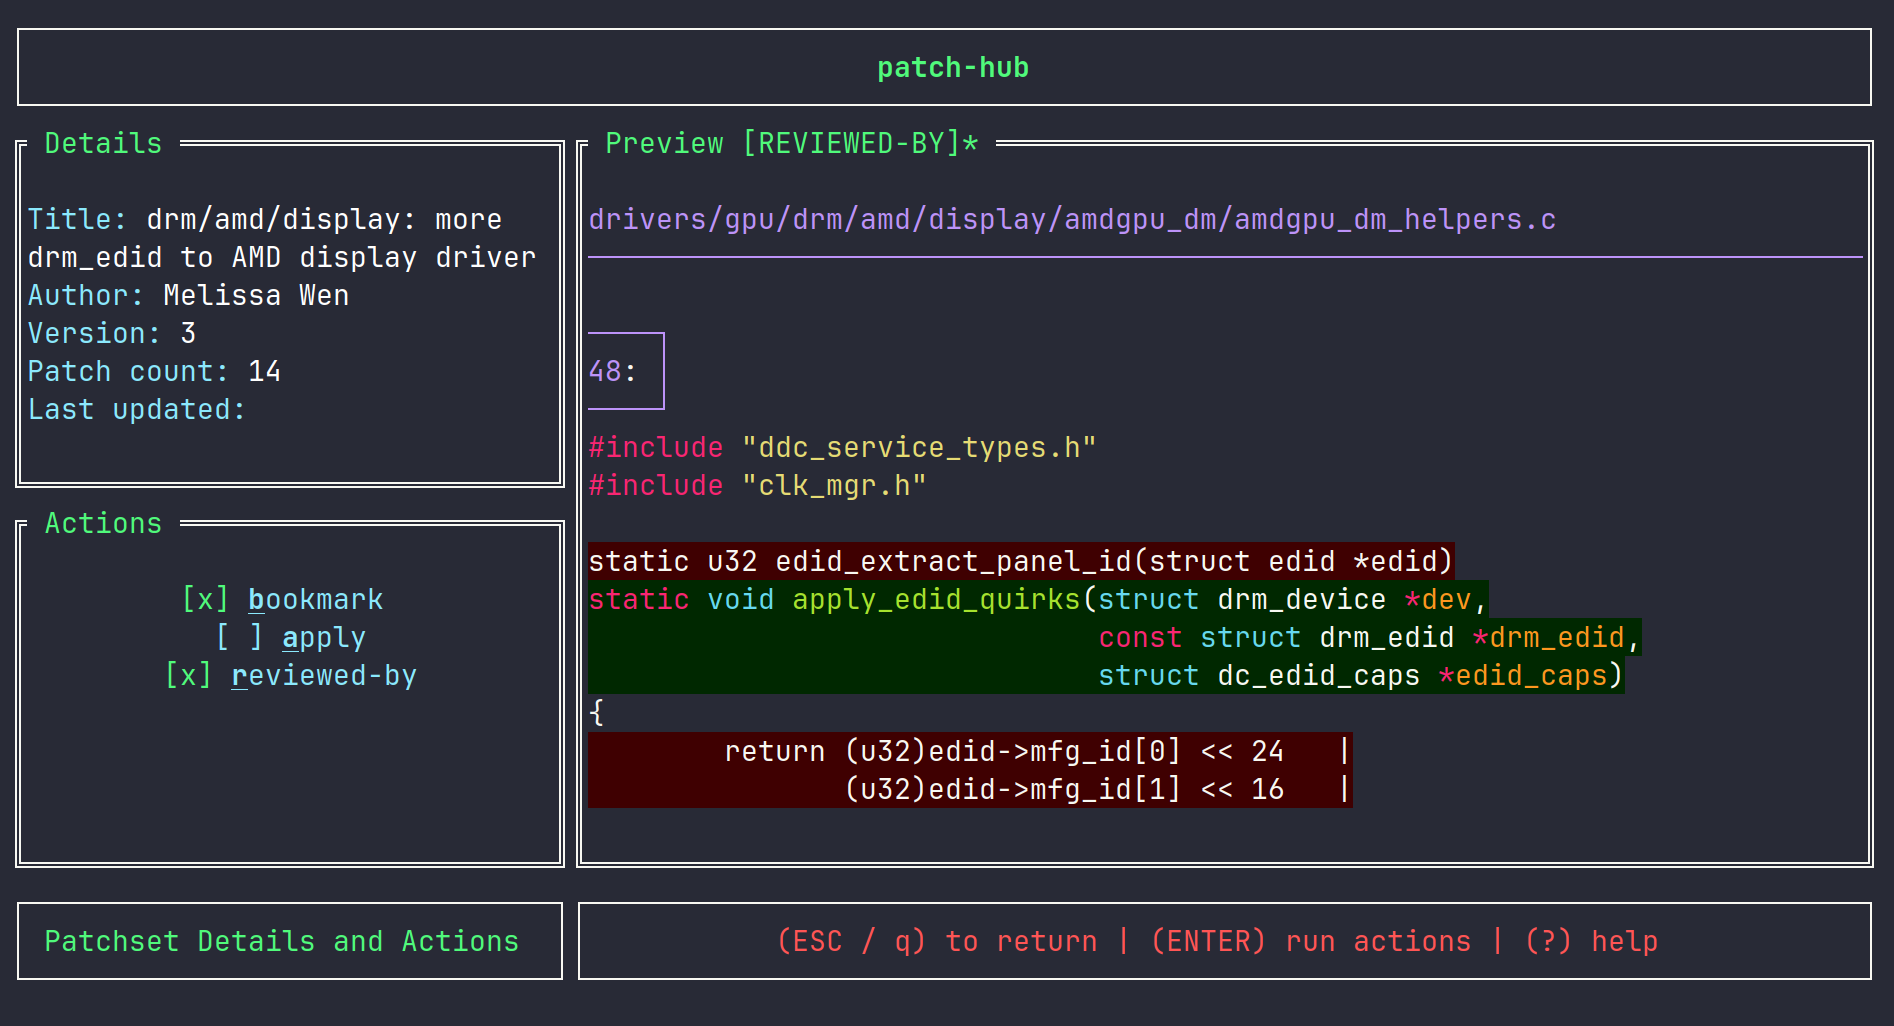
\includegraphics[width=1\linewidth, 
    clip=true, trim= 0px 0px 0px 0px]
    {figs/kw_patch_hub_example}}
    \caption{\texttt{kw patch-hub} use case.}
    \label{fig:patchset-dev-workflow}
\end{figure}

\subsection{Project architecture}

Describing kw as hub-like fits not only from the user's perspective, as it is a
collection of diverse features in a unified interface, but also from the project
developer's perspective. The project code base is structured as follows:

\begin{enumerate}
	\item Entry point file named \texttt{kw} located at the root of the
	repository~\cite{kworkflow-entrypoint}, that is our \textit{hub} component;
	\item Feature-specific files named after their respective feature (e.g., the
	\texttt{build} feature has the \texttt{build.sh} file) located at the
	\texttt{src/} directory~\cite{kworkflow-features}. These are our
	\textit{features} components;
	\item Library files named after their scope (e.g., \texttt{kw\_string.sh}
	deals with string manipulations) located at the \texttt{src/lib/}
	directory~\cite{kworkflow-libraries}, that are shared across
	feature-specific files. These are our \textit{libraries} components;
	\item Plugin files with code heavily coupled with specific distros, CPU
	architectures, subsystems, and the like, that can change externally and are
	very mutable, located at the \texttt{src/plugins/}
	directory~\cite{kworkflow-plugins}.  These are our \textit{plugins}
	components
\end{enumerate}


As an illustration of kw's inner workings, let us simulate an execution of a
\texttt{kw deploy} call. First, the entry point \texttt{kw} file is loaded and
executed. At the beginning, global variables are dynamically defined, then using
a switch-case, we resolve the feature as \texttt{deploy}, load the
\texttt{deploy.sh} file, and call the standard main function of feature-specific
files (in this case, \texttt{deploy\_main()}). This function handles the rest of
the \texttt{deploy} execution, using other functions defined inside
\texttt{deploy.sh} and leveraging functions from the libraries and plugins
components.

\begin{figure}[htbp]
    \centering
    \fbox{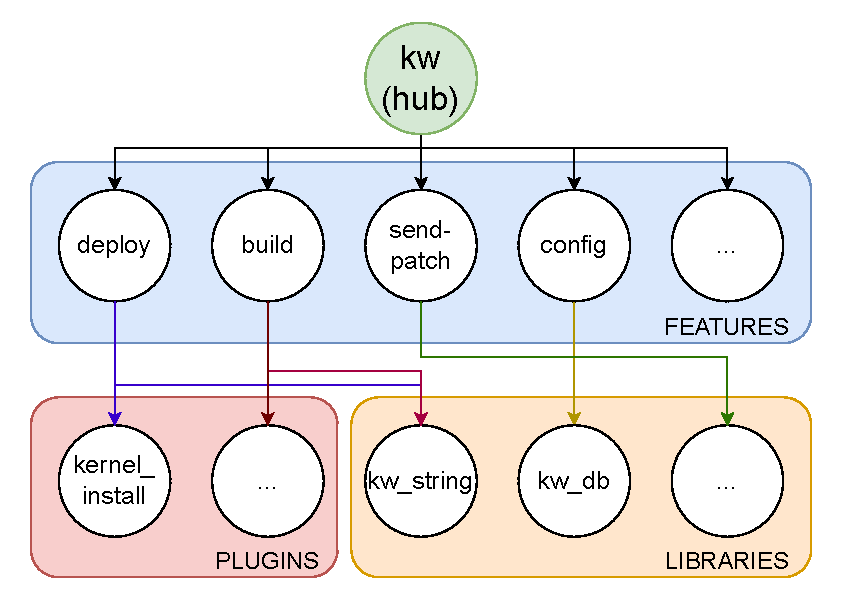
\includegraphics[width=0.8\linewidth, clip=true, trim= 0px 5px 0px 5px]
    {figs/kw-architecture.pdf}}
    \caption{kw conceptual architecture.}
    \label{fig:kw-arch}
\end{figure}

The diagram in \textbf{Figure~\ref{fig:kw-arch}} models kw's architecture
showing how extensible and modularized the project is. Note that this diagram is
for illustration purposes and does not reflect the precise load and execution
relation of features and libraries/plugins.

\subsection{Data collection for scientific research}

Inside the kw project, we have implemented an infrastructure to collect
statistics and other data, along with a lightweight and single-file database
using \textit{SQLite3}~\cite{sqlite}. For instance, every time a developer builds
a kernel, the time it took for the compilation is captured (using the
\texttt{statistics} library) and registered in kw's database (using the
\texttt{kw\_db} library). This type of data collection happens in other places
across kw, but many other data points opportunities can be used to conduct
further scientific research on kernel workflows.

To name a few, kw captures: build and deploy times, logging if they were
successful; target machine kernel list and uninstall events. We can also list
some data points of interest in terms of research on the kernel workflows:
during build, capture hardware specifications and cross-compilation strategies,
enabling analysis of efficient hardware setups and common compiler use; during
deployment, record target distro, bootloader, and deployment method, which can
uncover the landscape in terms of testing environments used; during patch
submission log maintainer/mailing list targeting, providing insights about
overloaded personell/subsystems in the Linux project hierarchy.

All data is stored locally in a single file within the user's file system, never
exfiltrated, and users can easily opt out by disabling data collection. We also
plan to implement a telemetry system for users to voluntarily submit data for
research, inspired by the \textit{Debian Popularity
Contest}~\cite{debian-popcon}, a standard in telemetry and anonymization.

\subsection{Comparison with other tools}

kw works as a hub-like tool that continuously incorporates existing robust tools
to avoid duplication, while also implementing features from scratch when no
existing tools (satisfiably) solve a given pain point. Incorporating other tools
involves adding our biases, which we believe are closely tied to the Linux
kernel development model rules and workflows. In this respect, no other tool
exists that proposes a similar all-in-one approach to mitigate bottlenecks in
kernel workflows, making kw a novel solution.

